\newpage
\chapter{Neural IR}
\label{chap:neurIR}

\section{Overview}

As previously stated, IR community has recently been very interested in neural network approaches, given the fact that they deliver state-of-the-art performance in many machine learning tasks (e.g., speech recognition, computer vision, and natural language processing), they may also be beneficial in IR tasks.

Relevant researches in the last period of time (2009 - 2016) has mainly been focused on the long standing vocabulary mismatch problem in textual IR \cite{neurIRearly}.

Guo et al. distinguished two categories of Neural IR models \cite{deeplookneurir} based on whether their target is learning words representation (to alleviate the first of the previous problems) or a ranking function (to alleviate the second problem): representation-focused models and interaction-focused models.

\textbf{Representation-focused} models assume that the relevance between a query and a document depends on their compositional meaning and, therefore, they focus on learning complex, high level representations of the input text (e.g. distributed representations, explained below).

\textbf{Interaction-focused} models assume that the relevance between a query and a document depends on relations between them and learning is thus achieved by looking at their interactions rather than finding complex representations.

These two categories are reflected in two architectures, reported in figure \ref{fig:neur2arch}. In the first part (A), queries and documents are separately passed through mirror (siamese) neural networks with shared parameters and scores are generated based on the combination of the respective outputs. By contrast, the second part (B) defines an approach in which a joint representation for queries and documents is constructed and then run through a neural network.

\begin{figure}
  \centering
  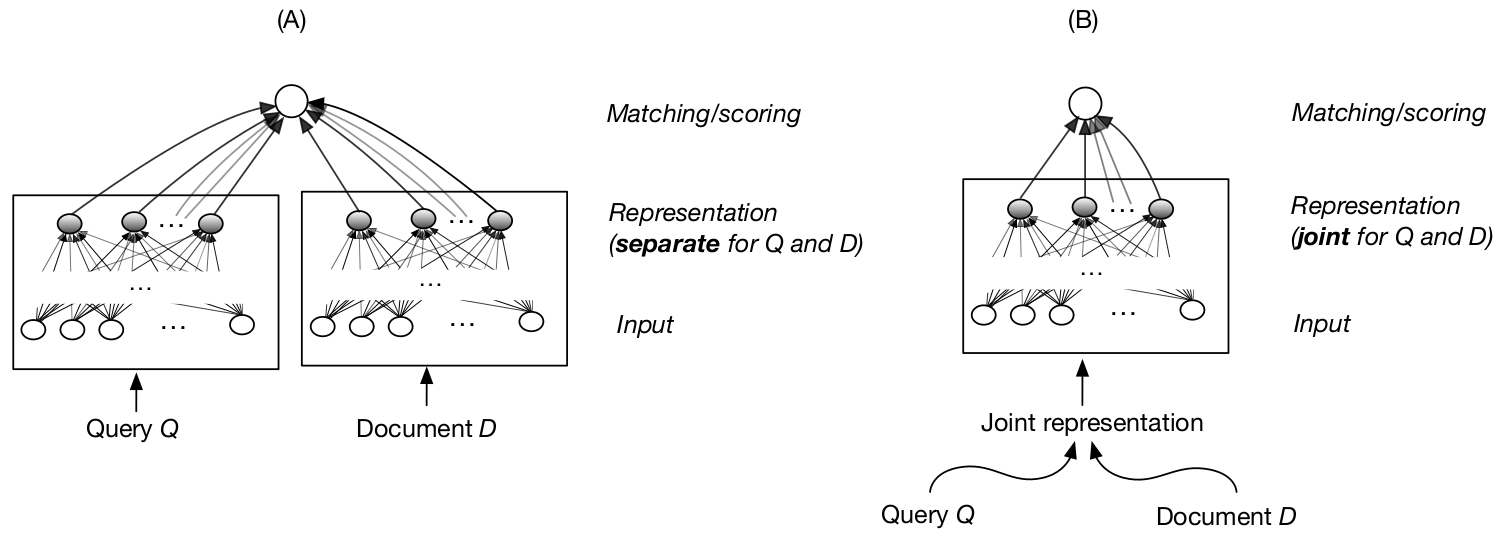
\includegraphics[width=1.0\textwidth]{neur2arch.png}
  \caption{Two basic neural architectures for scoring the relevance of queries to documents: (A) representation-focused model and (B) interaction-focused model (picture taken from \cite{neurIRearly})}
  \label{fig:neur2arch}
\end{figure}

Alongside with these two approaches, Onal, Zhang et al. in \cite{neurIRearly} described two categories in which neural techniques and distributed representations can be used together to build a model for an IR task: \textit{aggregate} and \textit{learn}.

In the first category, \textit{aggregate}, the models rely on pre-trained word representations as external  resources in order to build or extend relevance matching functions.

In the second category, \textit{learn}, the models are  designed and trained  to learn ``good'' word representations  and  semantic compositionality functions for building distributed representations from scratch, given only raw text.

The approaches of the second category may vary upon the training objectives defined:

\begin{itemize}
    \item \textit{learn to autoencode}, where the training objective  is to restore  the  input based on the distributed representation learned by a neural network;
    \item \textit{learn to match} (under supervised learning), where the training objective is to minimize a loss function, given a neural network that computes a degree of similarity between a query and a document;
    \item \textit{learn to predict}, which refer to neural language models used for learning representations of larger textual units (e.g. sentences, paragraphs, documents) from unlabelled data - and
    \item \textit{learn to generate}, where a synthetic textual unit is generated based on the distributed representation of an input text.
\end{itemize}

The work studied and reproduced in this thesis belongs to the second category, more specifically, to \textit{learn to match}.

Typically, interaction-focused and learn to match approaches are conducted under supervised learning while all the other are fall into unsupervised learning.

The proportion of labelled and unlabelled data that is available influences the level of supervision that can be employed for training a deep Neural IR model.

Since it is difficult to obtain large amounts of supervised data, when click information in click-through logs are available, they are exploited to derive similarity assessments for query-document pairs.

Moreover, if few labelled data are available, then they can be leveraged to train a retrieval model with few parameters that in turn uses text representations that is pretrained on larger unlabelled corpus (semi-supervised approach).

Much of the explorations in Neural IR models have focused on learning good representations of text \cite{nn4ir}. However, these representation learning models tend to perform poorly when dealing with rare terms.

Based on similar motivations, the authors of the model reproduced in this thesis have recently emphasized the importance of modelling lexical matches using deep neural networks.

The majority of neural ranking models are implemented as multistage rankers: since most of them rely on semantic matching that can be achieved using distributed dense representations, computing the retrieval score for all the documents in a large-scale collection is generally infeasible.

Zamani et al. states in \cite{stdlnneur} that the representations of documents and queries are what makes the traditional term based ranking models fast, and the neural ranking models slow.

This strategy, where different IR models are chained to re-rank a smaller number of candidate documents is called \textbf{telescoping evaluation} in \cite{nn4ir}.

Telescoping evaluations are common in the Neural IR literature, where a neural model only re-ranks the top ranked documents retrieved by a first-stage efficient ranker in response to a given query.

The reliance on a first stage ranker creates a dual problem: first, the interaction and combination effects are not well understood. Second, the first stage ranker serves as a ``gate-keeper'' or filter, blocking the potential of neural models to uncover new relevant documents.

Moreover, Mitra et al. in \cite{Mitra2016ADE} demonstrate that good performances on re-ranking tasks may not be indicative how a neural retrieval model would perform if the retrieval involves larger document collections. They found that, in that case, their embeddings-based approach (DESM) was prone to false positives, retrieving documents that are only loosely related to the query.

To counteract this fact, they defined a ``mixture'' model - a linear combination of a neural retrieval model and a traditional retrieval model (DESM + Bm25) - and evaluated it in a non-telescoping setting. The mixture model provided improvements over the performance of DESM alone.

\subsection{A brief history of Neural IR}
\label{ssec:historyNeuIR}

The first successful Neural IR model was the Deep Structured Semantic Model (DSSM) \cite{dssm}, introduced in 2013, which is a supervised neural ranking model that  directly  tackles  the  ad-hoc  retrieval  task. In the same year, Lu and Li proposed DeepMatch \cite{deepmatch}, which is a deep matching method applied  to the Community-based Question Answering (CQA) and micro-blog matching tasks.

At the same time, there was a number of studies focused on learning low-dimensional representations of text with and unsupervised neural approach; the most known model of them is \textit{Word2Vec} \cite{w2v}.

Later, between 2014 and 2015, work on neural ranking models began to grow, bringing new variants of DSSM \cite{cdssm}, ARC-I \cite{arc}, ARC-II and MatchPyramid. Methods to compose word embeddings over long textual units were also proposed (e.g. Paragraph Vector \cite{pv}).

Moreover, in 2014, the first two Neural IR papers also appeared at SIGIR.

In 2016, work on Neural IR continued to accelerate in quantity of work, sophistication of methods, and practical effectiveness (e.g. \cite{drmm} - the work studied and reproduced in this thesis). SIGIR also featured its first workshop on the subject \footnote{\url{https://www.microsoft.com/en-us/research/event/neuir2016}}.

With respect to the test collection used in the experimental section (Robust04 \cite{rob04}) (\ref{sec:leaderboadrobust04}), I explored a neural model that demonstrate state-of-the-art performances, published after DRMM.

In 2018, Zamani et al. proposed in \cite{stdlnneur} a \textit{standalone} neural ranking model (SNRM) that addresses the inefficiency problems of neural models by enforcing and rewarding sparsity in the representation learning, creating a latent representation that aims to capture meaningful semantic relations while still matching documents.

SNRM aim is learning highly sparse representations for documents and queries that result in better matching compared to the dense term vectors and exact matching models. It can also take advantage of pseudo-relevance feedback for further improvements.

Limited training data has been a perennial problem in IR, and many machine learning-related domains. This has motivated researchers to explore building models using pseudo-labels. For example, pseudo-relevance feedback (PRF) assumes that the top retrieved documents of a previous search result in response to a given query are relevant.

Although this assumption does not necessarily hold, PRF has been proven to be effective in many retrieval settings.

Onal et al. in \cite{neurIRearly} reviewed a huge amount of works and drew some interesting conclusions about Neural IR, along with some criticisms.

While neural networks methods have worked quite well on short texts, effectiveness on longer texts typical of ad-hoc search has been problematic with only very recent evidence to the contrary \cite{drmm}.
 
Side by side comparisons of lexical versus neural methods often show at least as many losses as gains for neural methods, with at best an advantage ``on average''.
 
In addition, deep structures with a very large number of hidden layers have typically been less effective in IR compared to their shallow counterpart.
 
When Neural IR has led to improvements in ad-hoc search results, improvements appear relatively modest when compared to traditional query expansion techniques for addressing vocabulary mismatch problem.

Query expansion (QE) is a process in IR which consists of selecting and adding terms to the user’s query with the goal of minimizing query-document mismatch and thereby improving retrieval performance; however it is not relevant w.r.t. the work in this thesis.

In \cite{deeplookneurir} Guo et al. argue that there is still a long way to go for neural ranking models: 1) they have not had the level of breakthroughs achieved by neural methods in speech recognition or computer vision; 2) there is little understanding and few guidelines on the design principles of neural ranking models; 3) special capabilities of neural ranking models that go beyond traditional IR models have not been yet identified.

\section{Text representations}

Neural models have shown their importance in learning ``good'', dense and small text representations.

The way queries and documents are represented is very important in IR, for their representations are the building blocks of the entire IR process.

In fact, different representations of a text raise different notions of similarity.

Two popular ways to represent textual data are the following:

\begin{itemize}
 \item \textbf{Local representation} (\textit{one-hot} encoding/representation): given a dictionary $\mathcal{V}$, a word is represented with a vector $\vec{v}$ with length $|\mathcal{V}|$.
All positions are 0 except for the position corresponding to that word (which is
set to 1); $\vec{v} \in \{ 0, 1\}^{|V|}$
 \item \textbf{Distributed representation}: given some features of text, a word is represented with a vector $\vec{v}$ of |features| positions with real values; $\vec{v} \in \mathcal{R}^{|features|}$
\end{itemize}

When the vectors are high-dimensional, sparse, and based on distributional features they are referred to as \textit{explicit vector representations}.

On the other hand, when the vectors are dense, small ($k<<|V|$), and learned from data then they are commonly referred to as \textbf{embeddings}.

In a distributed representation the feature space is very important because it influences the notion of similarity captured.

Popular features used are distributional properties of terms (e.g., document term frequency, neighboring terms with or without distances, etc.) and different weighting schemes (e.g., TF-IDF) applied over the raw counts.

\subsection{Distributed representation}

The idea of distributed representations originated from the work of John Rupert Firth who was an English linguist and a leading figure in British linguistics during the 1950s.

Firth studied the context-dependent nature of meaning and described it as ``context of situation''. He is known for the famous quotation:

\begin{quote}
``You shall know a word by the company it keeps'' \cite{firth}
\end{quote}

This theory implies that a desirable property is that the representation of a word should be similar to the representations of the words surrounding it.

Both distribution and semantics by themselves are not well-defined and under different context may mean very different things.

In fact, they are very dependent by the distributional properties chosen as features, which in turn influence the notion of similarity.

For instance, let's consider three different features space based on the following properties (respectively): (a) presence or absence of the term in a document; (b) neighbouring words in a window and (c) neighbouring words with distance.

If one considers the sentence ``Time flies like an arrow; fruit flies like a banana'' then, the distributed representations of the term ``banana'' are shown in figure \ref{fig:banana}.

\begin{figure}
  \centering
  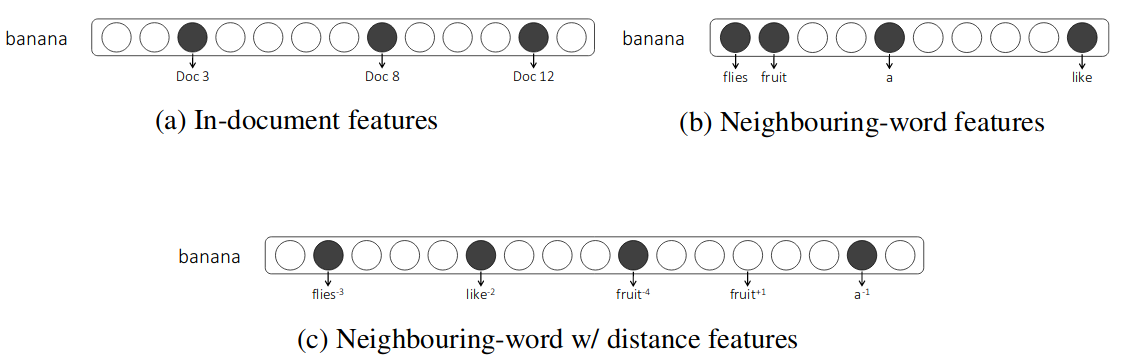
\includegraphics[width=0.9\textwidth]{banana.png}
  \caption{Examples of different feature-based distributed representations of the term ``banana'' (picture taken from \cite{nn4ir})}
  \label{fig:banana}
\end{figure}

In \cite{nn4ir}, Mitra and Craswell refer to two notions of similarity: \textbf{typical} (two words that belong to the same class/type - e.g. capital cities names) and \textbf{topical} (two words that are related to the same topic - e.g. a writer and its publications).

They state that representations like (a) yield a notion of topical similarity while representations like (c) yield a notion of typical similarity. (b)-like representations yield a mixture of topical and typical similarity.

In the context of neural models, distributed representations generally refer to learnt embeddings.

Common approaches for learning embeddings include either factorizing one of the matrix presented in the following section (e.g. with LSA) or using gradient descent based methods that try to predict some features given the term (e.g. \textit{Global Vectors} GloVe \cite{Glove} - GloVe is an unsupervised learning algorithm for obtaining vector representations for words \url{https://nlp.stanford.edu/projects/glove/} - or Word2Vec).

The query and the document embeddings themselves can be compared using a variety of similarity metrics, such as cosine similarity or dot-product.

A study \cite{ewr} shows that, similarly to the neural embedding space, the explicit vector space also encodes a vast amount of relational similarity which can be recovered in a similar fashion (although it is more expensive in terms of size).

What's interesting about this work is that it implies that the neural embedding process is not discovering novel patterns, but rather is doing a remarkable job at preserving the patterns.

\section{Models for semantic matching}
\label{sec:modelsSemantic}

The terms distributional, corpus-based or statistical all refer to a family of approaches to semantics that share the
assumption that the statistical distribution of words in context plays a key role in characterizing their semantic behavior.

\begin{quote}
Statistical patterns of human word usage can be used to figure out what people
mean.

- \textbf{Statistical semantics hypothesis} (SSH)
\end{quote}

This general hypothesis underlies several more specific hypotheses, such as the distributional hypothesis, the extended distributional hypothesis and the latent relation hypothesis, discussed below.

\subsection{Similarity of documents: the term-document matrix}

Given a corpus $C$, the term-document matrix $A$ represents the relation (based on a feature (function) $f$) between unique terms and documents in $C$.

Let $m$ be the number of unique terms and let $n$ be the number of documents in $C$. Then, $A$ has size $m\cdot n$.

Let the feature considered be the frequency. Then, each row $a_{i,}$ contains
the frequencies of a term $t_i$ over the corpus $C$ (\textit{signature of $t_i$}),
and each column $a_{,j}$ contains the frequencies of all $m$ terms over the document $d_j$ (\textit{signature of $d_j$}).

\begin{equation}
\label{eq:tdmatrix}
A = \begin{bmatrix}
    & d_1 & d_2 & \dots & d_n \\
    t_1 & f_{11} & f_{12} & \dots & f_{1n} \\
    t_2 & f_{21} & f_{22} & \dots & f_{2n} \\
    \vdots & \vdots & \vdots & \ddots & \vdots \\
    t_m & f_{m1} & f_{m2} & \dots & f_{mn} \\
    \end{bmatrix}
\end{equation}

If two documents have similar topics, then the two corresponding column vectors
will tend to have similar patterns of numbers (SSH).

A popular representation that implements this notion of similarity is called \textbf{Bag Of Words} (BOW) representation. It is called \textit{bag} of words because any information about the order or structure of terms in the documents is discarded.

\subsection{Similarity of words: the term-context matrix}

\begin{quote}
The distributional hypothesis in linguistics is that words that occur in
similar contexts tend to have similar meanings.

- \textbf{Distributional semantics hypothesis} \cite{harris}
\end{quote}

Therefore, according to the DSH, at least certain aspects of the
meaning of lexical expressions depend on the distributional properties of such
expressions, i.e. on the linguistic contexts in which they are observed.

The term-context matrix $B$ is similar to the term-document matrix, with the
distinction that columns are context $c$ of words. Row and column vectors now
have both length equal to the size of the vocabulary.

\[
B = \begin{bmatrix}
    & c_1 & c_2 & \dots & c_m \\
    t_1 & f_{11} & f_{12} & \dots & f_{1m} \\
    t_2 & f_{21} & f_{22} & \dots & f_{2m} \\
    \vdots & \vdots & \vdots & \ddots & \vdots \\
    t_m & f_{m1} & f_{m2} & \dots & f_{mm} \\
    \end{bmatrix}
\]

The size of the context window determines the count in each position of the matrix as well as its sparseness.

Whit a short context window the representation of words captures a syntactic notion of similarity, viceversa with a long context window the representation of words is likely to capture their semantic meaning.

The output of a distributional model is a distributed representation.

\subsection{Similarity of relations: the pair-pattern matrix}

In a pair-pattern matrix, the columns represent the patterns (e.g. X works with
Y) and the rows represent the pairs (e.g. blacksmith:iron).

The \textbf{extended distributional hypothesis} states that patterns that
co-occurs with similar pairs tends to have similar meaning (e.g.
carpenter:wood co-occurs in the pattern X works with Y and X cuts Y. Both
patterns could be represented with the relationship artisan:material).

The \textbf{latent relation hypothesis} states that pairs that co-occurs with
the same patterns have similar semantic relationship. This is the inverse of the
previous hypothesis (e.g. carpenter:wood and blacksmith:iron co-occur in
X works with Y, so carpenter's relationship with wood is similar to
blacksmith's relationship with iron).

To sum up, pair-pattern matrices are suited to measuring the similarity of
semantic relations between pairs of words; that is, relational similarity.

In contrast, word-context matrices are suited to measuring attributional
similarity.

\section{Word embeddings}

An important consideration here is the choice of the term embeddings that is appropriate for the retrieval scenario.

It is important to understand how the notion of inter-term similarity modelled by a specific vector space may influence its performance on a retrieval task

Models that consider term-document pairs generally capture topical similarities in the learnt vector space.

On the other hand, models like Word2Vec \cite{w2v} and GloVe \cite{Glove} capture a mixture of topical and typical notions of relatedness.

Embedding based models often perform poorly when the retrieval is performed over the full document collection; however the errors made by embedding based models and exact matching models may be different—and the combination of the two is often preferred.

For example, an exact matching model may be tricked if some query term are in a non-relevant document and an embedding based model may be tricked if a non relevant document is topically (or typically) close to a query term.

\subsection{Word2Vec: unsupervised approach to learn term representations (exploiting semantic models)}

Mikolov et al. proposed in \cite{w2v} two main Word2Vec models: 

\begin{itemize}
 \item Continuous Bag of Words (CBOW), that predicts a word given the context;
 \item Skip-Gram, which predicts the context given a word.
\end{itemize}

Word2Vec is part of the \textbf{``Neural Probabilisitic Language Models (NPLMs)''} family, also known as \textit{context-predicting} models.

A NPLM represents each word in the vocabulary as a vector $\vec{x} \in \mathbb{R}^n$ and defines the scoring function $s_{\theta}$ in terms of vectors of the context words and the next word.

In these models, a neural network tries to predict co-occurrence likelihood of context-word pairs. Such probability $P(w_t | w_c)$, given a target word $w_t$ corresponding to a context $w_c$ is computed by the \textit{softmax function}:

\begin{equation}
P(w_t | w_c) = softmax(w_t, w_c) = \frac{exp(s_{\theta}(w_t,w_c))}{\sum_{w' \in \mathcal{V}} exp(s_{\theta}(w', w_c))}
\end{equation}

where $\mathcal{V}$ is the vocabulary and $s_{\theta}$ is the scoring function (the neural network), with $\theta$ as parameters, that quantifies the compatibility of word $w_t$ with context $w_c$.

The softmax function is another non-linear activation function which output is obtained by considering information about all set of input elements, not just one (e.g. sigmoid). The output values of softmax are in the range $[0,1]$ and sum up to 1.

It is often used to turn an arbitrarily large or small numbers into a probability distribution.

\subsubsection{Word2Vec: CBOW model}

CBOW aim to predict a word $w_t$ from the context $w_c$

\begin{figure}[H]
  \centering
  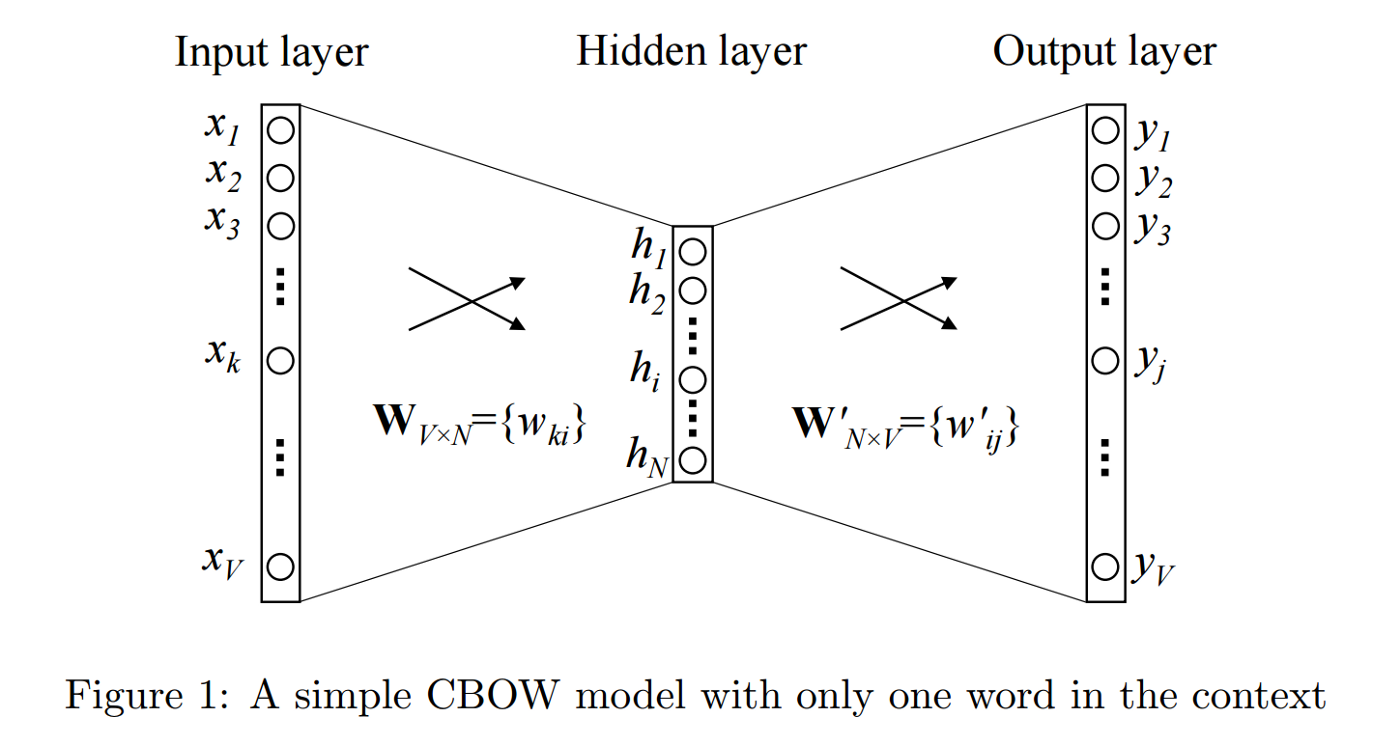
\includegraphics[width=0.7\textwidth]{embeddings.png}
  \caption{CBOW simple model (context = 1 word) (reference image \cite{w2ve})}
  \label{fig:emb}
\end{figure}

Let vocabulary size be $|\mathcal{V}| = V$ and embeddings size be N. The context $w_c$ surrounding the target word $w_t$ is a hot vector $x_1, ..., x_n$.

This vector is compressed in the hidden layer $h=x^T \cdot W$, then it is decompressed to obtain a score $u = W'^t \cdot h$ that is a measure of the match between the context and the target word.

Finally the posterior probability of each word is calculated, i.e. the probability that the output word is equal to the target word (softmax function is applied to $u$):

\begin{equation}
p(w_t | w_c) = y_t = softmax(u_t) = \frac{e^{u_t}}{\sum_i^V e^{u_i}}
\end{equation}

The aim of this model is to maximize such probability (the loss function needs
to evaluate the output vector $u$ at the ideal index $t$):

\begin{equation}
\begin{split}
\max p(w_t | w_c) &= \max y_t \\
&= \max log(y_t) \\
&= \max log(softmax(u_t)) \\
&= \max log \left( \frac{e^{u_t}}{\sum_i^V e^{u_i}} \right) \\
&= - u_t + \sum_i^V e^{u_i}
\end{split}
\end{equation}

So, the loss function is:

\begin{equation}
\mathcal{L} = - u_t + \sum_i^V e^{u_i}
\end{equation}

The softmax function requires that the probability $e^{u_t}$ is normalized by summing over all the vocabulary, which is an expensive computation to do in case of large corpus. Thus, to make the model scalable, the authors proposed a sightly altered \textbf{negative sampling} objective:

\begin{equation}
\mathcal{L} = - u_t + \sum_i^N e^{u_i}
\end{equation}

where N is the number of negative sample words drawn either from the uniform or empirical distribution over the vocabulary.

This model can be generalized with multiple context words; in fact the general form is used for the creation of word embeddings in later experiments of this thesis.

\subsubsection{Word2Vec: Skip-Gram}

Skip-Gram is the opposite of CBOW: in Skip-Gram the context $w_c$ is predicted given an input word $w_t$.

Basically the training objective of the Skip-Gram model is to learn word
vector representations that are good at predicting nearby words in the
associated context.

At the output layer, instead of outputting one multinomial distribution,
the output consists of $|w_c|$ multinomial distributions. Each output is computed using the same hidden layer.

The output of the model is the probability that the prediction of the j-th word on
the c-th panel, $w_{c,j}$ , equals the actual word, conditioned on the input word $w_t$.

\begin{equation}
p(w_{c, j} | w_t) = \frac{exp(u_{c, j})}{\sum_{j' = 1}^V exp(u_{c,j'})}
\end{equation}

\begin{figure}[H]
  \centering
  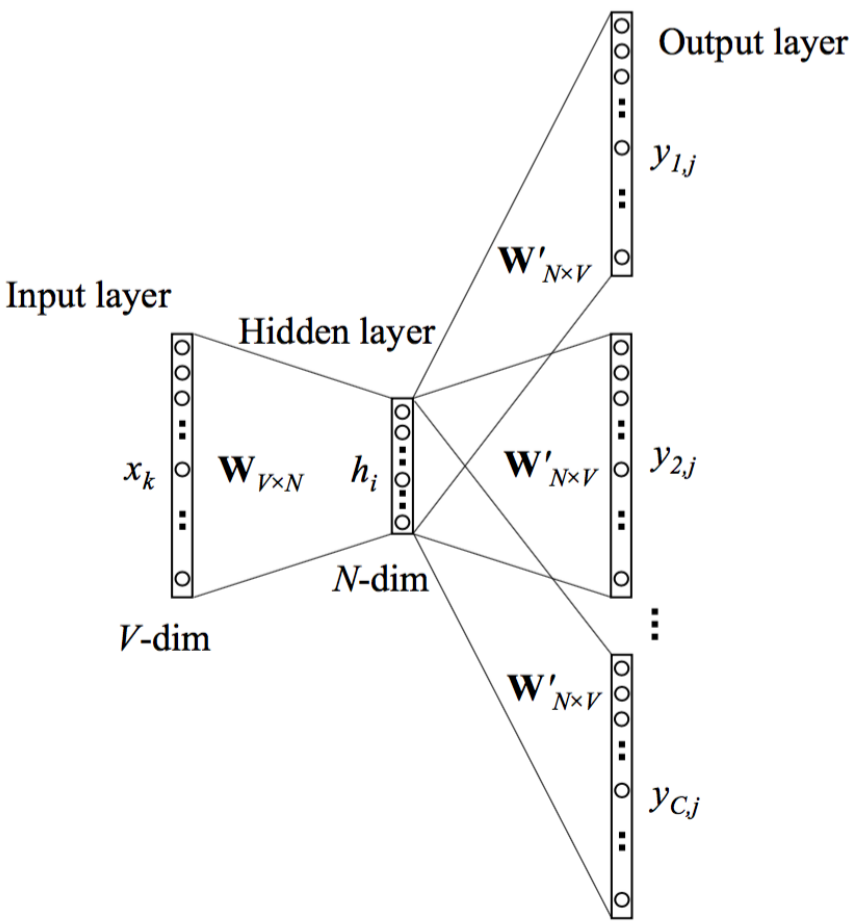
\includegraphics[width=0.6\textwidth]{skip-gram.png}
  \caption{Skip-gram model (reference image \cite{w2ve})}
  \label{fig:skip-gram}
\end{figure}

Word2Vec model's output consists of two different weight matrices: $W$ (IN-embeddings) and $W'$ (OUT-embeddings). Generally, only $W$ is used and $W'$ is discarded after training.

\subsection{On the importance of word embeddings}
The usage of word embeddings comes with its own challenges and decision problems.

For instance, some decisions to be considered are the choice of the possible algorithms: Word2Vec (cbow or skip-gram) \cite{w2v} or GloVe the choice of hyper-parameters (e.g., dimensionality of embedding space, window size, etc.) and the choice of training data/corpora.

Does performance vary much if pre trained embeddings are used vs. re-training embeddings for a target domain, either by fine-tuning pre trained embeddings or re-training from scratch? How should one deal with out-of-vocabulary (OOV) query terms not found in the word embedding training data for query-document matching?

Some studies gave empirical answers to these questions. In \cite{neurev} it is reported a number of studies that found no significant difference between Word2Vec or GloVe, skip-gram of cbow.

In the same review study, there are discording results on the impact of training corpus for word embeddings: some found that when the background training corpus matched the target corpus from a topical point of view, the performance improved; other found that the choice of corpus used to construct word embeddings had little effect on retrieval results.

Regarding the handling of OOV terms, some solutions proposed were to ignore the OOV terms or to randomly initialize their embeddings.

Mitra et al. in \cite{Mitra2016ADE} explored the possibility to combine both in-embeddings and out-embeddings of Word2Vec (usually discharged after training) in order to explore different topic-based relationship between a query and its relevant documents.

For instance, table \ref{tab:embsim} shows that in-in and out-out cosine similarities are high for words that are similar by function or type (typical), and the in-out cosine similarities are high between words that often co-occur in the same query or document (topical).

\begin{table}[H]
\centering
\begin{tabular}{cc}   % top level tables, with 2 rows
\begin{tabular}{ccc}
\hline
\multicolumn{3}{c}{\textbf{yale}} \\
in-in & out-out & in-out \\ \hline
yale & yale & yale \\
harvard & uconn & faculty \\
nyu & harvard & alumni \\
cornell & tulane & orientation \\
\hline
\end{tabular} &
\begin{tabular}{ccc}
\hline
\multicolumn{3}{c}{\textbf{eminem}} \\
in-in & out-out & in-out \\ \hline
eminem & eminem & eminem \\
rihanna & rihanna & rap \\
ludacris & dre & featuring \\
kanye & kanye & tracklist \\
\hline
\end{tabular}
\end{tabular}
\caption{Tables with data reported by Mitra et al. in \cite{Mitra2016ADE}. They shows nearest neighbours for the words ``yale'' and ``eminem'' according to the cosine similarity based on the in-in, out-out and in-out embeddings. Their Word2Vec model was trained on a query corpus with a vocabulary of 2748230 words}
\label{tab:embsim}
\end{table}

They proposed a ``Dual Embedding Space Model'', with one embedding for query  words and a separate embedding for document words, learned jointly based on an unlabelled text corpus.

Recently, Zamani and Croft in \cite{relbasedwe}, point out that embedding vectors used in Neural IR are typically learned based on term proximity in a large corpus. In Word2Vec, for instance, the objective is to predict adjacent word/s for a given word or context. They argue that such objectives (based on term proximity, syntactic, or even semantic similarity) is not is not necessarily equivalent to capture relevance.

The following example shows this fact: let ``dangerous vehicles'' be a query submitted by a user. One of the most similar terms to this query based on the typical word embedding algorithms (e.g., Word2Vec and GloVe) is ``safe'', and thus it would get a high weight in the expanded query model. The reason is that the words ``dangerous'' and ``safe'' often share similar contexts. However, expanding the query with the word ``safe'' could lead to poor retrieval performance, since it changes the meaning and the intent of the query. This can be seen in a later example (\ref{fig:cos_sim_sample}), where ``crime'' is similar to ``justice''. For the same reason, Word2Vec fails on the notion of antonymy: words with opposite meanings are actually very likely to occur in similar contexts,

In \cite{relbasedwe}, Zamani and Croft developed two learning models with different objective functions; one that learns a relevance distribution over the vocabulary set for each query and the other that classifies each word as belonging to the relevant or non-relevant class for each query.

They used a technique similar to PRF to train their models. Contrary to PRF, they used an offline approach (without the need of an extra retrieval run) in which they considered a fixed-length dense vector for each vocabulary term and estimate these vector based on the information extracted from the top retrieved documents for large numbers of training queries.

They reported that the relevance-based word embedding models outperform state-of-the-art word embedding algorithms, and showed that the expansion terms chosen by their models are related to the whole query, while those chosen by typical word embedding models are related to individual query term.
